% main.tex

% Use the ACM large 1-column format class from your template directory
\documentclass[acmlarge]{template/column-format-template/acmart}

% Set up any additional package imports here
\usepackage{graphicx}     % For including graphics
\usepackage{amsmath}      % For advanced math formatting
\usepackage{algorithm}    % For algorithm pseudocode
\usepackage{algorithmic}  % For algorithm pseudocode
\usepackage{booktabs}     % For professional tables
\usepackage{listings}     % For code listings
\usepackage{subcaption}   % For subfigures
\usepackage{url}          % For URLs in bibliography
\usepackage{titlesec}     % For custom formatting
\usepackage{xcolor}       % For colors
\usepackage{listings}     % For code snippets
\usepackage{subcaption}   % For ...

% Custom settings for listings
\lstset{
    language=Python,                    % Sets the programming language for syntax highlighting
    basicstyle=\footnotesize\ttfamily,  % Sets the font style and size for the code
    keywordstyle=\color{blue},          % Style applied to keywords (e.g., "def", "import")
    commentstyle=\color{gray},          % Style applied to comments (e.g., lines starting with "#")
    stringstyle=\color{red},            % Style applied to strings (e.g., text within quotes)
    % backgroundcolor=\color{gray!10},  % Background color for the code block (light gray in this case)
    % numbers=left,                     % Displays line numbers on the left side of the code block
    % numberstyle=\tiny,                % Font size/style for line numbers
    % stepnumber=1,                     % Line number increment (e.g., every 1 line gets a number)
    % numbersep=5pt,                    % Distance between the line numbers and the code
    linewidth=0.95\linewidth,           % Code block occupies 80% of text width
    xleftmargin=-20pt,                  % Moves the listing 20pt closer to the left margin
    xrightmargin=5pt,                   % Optional: Adds extra padding on the right
    breaklines=true,                    % Automatically breaks long lines to fit within the page width
    captionpos=b,                       % Places the caption below the code block
    abovecaptionskip=5pt,               % Adjusts the space above the caption to 5pt
    belowcaptionskip=8pt,               % Adjusts the space below the caption to 8pt
}

% Remove ACM-specific references and permissions
\setcopyright{none} % Disable copyright
\makeatletter
\@printpermissionfalse
\@printcopyrightfalse
\@acmownedfalse
\makeatother

% Remove ACM reference format
\settopmatter{printacmref=false}
\renewcommand\footnotetextcopyrightpermission[1]{}

% Optional: Plain page style
\pagestyle{plain}

% TODO: check
% \BibTeX command to typeset BibTeX logo in the docs
\AtBeginDocument{%
  \providecommand\BibTeX{{%
    Bib\TeX}}}

% TODO: check
% Define paths for graphics and bibliography
% \graphicspath{{template/column-format-template/}}
% \bibliographystyle{template/column-format-template/ACM-Reference-Format}

% TODO: check
% \graphicspath{{figures/}}                 % Single directory
% \graphicspath{{fig1/}{fig2/}}             % Multiple directories

% TODO: check
% \bibliographystyle{ACM-Reference-Format}  % Standard ACM format
% \bibliographystyle{plain}                 % Basic format
% \bibliographystyle{ieeetr}                % IEEE format

% Optional: Customize section titles
% \titleformat{\section}
%   {\LARGE}                      % Large, not bold
%   {\thesection}                 % Section number
%   {0.5em}                       % Space between number and title
%   {}                            % Code before title body

% Optional: Customize subsection titles
% \titleformat{\subsection}
%   {\Large}                      % Large (but smaller than section), not bold
%   {\thesubsection}              % Subsection number
%   {0.5em}                       % Space between number and title
%   {}                            % Code before title body

% Optional: Adjust spacing before and after sections
% \titlespacing*{\section}{0pt}{2.5ex plus 1ex minus .2ex}{1.5ex plus .2ex}
% \titlespacing*{\subsection}{0pt}{2.25ex plus 1ex minus .2ex}{1.5ex plus .2ex}

\begin{document}

% Title
\title{SSH Shell Attacks}

% Define authors and their affiliations

\author{Andrea Botticella}
\authornote{The authors collaborated closely in developing this project.}
\email{andrea.botticella@studenti.polito.it}
\affiliation{%
  \institution{Politecnico di Torino}
  \city{Turin}
  \country{Italy}
}

\author{Elia Innocenti}
\authornotemark[1]
\email{elia.innocenti@studenti.polito.it}
\affiliation{%
  \institution{Politecnico di Torino}
  \city{Turin}
  \country{Italy}
}

\author{Renato Mignone}
\authornotemark[1]
\email{renato.mignone@studenti.polito.it}
\affiliation{%
  \institution{Politecnico di Torino}
  \city{Turin}
  \country{Italy}
}

\author{Simone Romano}
\authornotemark[1]
\email{simone.romano@studenti.polito.it}
\affiliation{%
  \institution{Politecnico di Torino}
  \city{Turin}
  \country{Italy}
}

% Short author list for page headers
\renewcommand{\shortauthors}{Botticella, Innocenti, Mignone, and Romano}

% CCS Concepts
\begin{CCSXML}
<ccs2012>
   <concept>
       <concept_id>10010147.10010257.10010321.10010337</concept_id>
       <concept_desc>Computing methodologies~Supervised learning by classification</concept_desc>
       <concept_significance>500</concept_significance>
   </concept>
   <concept>
       <concept_id>10010147.10010257.10010321.10010335</concept_id>
       <concept_desc>Computing methodologies~Unsupervised learning</concept_desc>
       <concept_significance>500</concept_significance>
   </concept>
   <concept>
       <concept_id>10010147.10010257.10010339</concept_id>
       <concept_desc>Computing methodologies~Natural language processing</concept_desc>
       <concept_significance>400</concept_significance>
   </concept>
   <concept>
       <concept_id>10010147.10010257.10010236</concept_id>
       <concept_desc>Computing methodologies~Machine learning</concept_desc>
       <concept_significance>400</concept_significance>
   </concept>
   <concept>
       <concept_id>10010147.10010528.10010531</concept_id>
       <concept_desc>Computing methodologies~Machine learning approaches</concept_desc>
       <concept_significance>300</concept_significance>
   </concept>
   <concept>
       <concept_id>10002978.10003006.10011634</concept_id>
       <concept_desc>Security and privacy~Intrusion detection systems</concept_desc>
       <concept_significance>200</concept_significance>
   </concept>
</ccs2012>
\end{CCSXML}

\ccsdesc[500]{Computing methodologies~Supervised learning by classification}
\ccsdesc[500]{Computing methodologies~Unsupervised learning}
\ccsdesc[400]{Computing methodologies~Natural language processing}
\ccsdesc[400]{Computing methodologies~Machine learning}
\ccsdesc[300]{Computing methodologies~Machine learning approaches}
\ccsdesc[200]{Security and privacy~Intrusion detection systems}

% Keywords
\keywords{Machine learning, supervised learning, unsupervised learning, language models, text classification, clustering, intent classification, SSH shell attacks, security log analysis}

% 00-abstract.tex

% Abstract: A concise summary of the project, including the main objectives, methods used, and key findings.

\begin{abstract}

% The exponential growth of cybersecurity threats has underscored the need for automated solutions to analyze and mitigate attack patterns. 
This paper introduces a comprehensive machine learning approach to analyze SSH shell attack sessions, leveraging both supervised and unsupervised learning techniques. Using a dataset of 230,000 unique Unix shell attack sessions, the methodology aims to classify attacker tactics based on the MITRE ATT\&CK framework and uncover latent patterns through clustering.

% \noindent Our approach employs robust pre-processing pipelines to transform unstructured textual logs into meaningful numerical representations, including Term Frequency-Inverse Document Frequency (TF-IDF) and embeddings from language models such as BERT and Doc2Vec. 
% Supervised classification experiments compare traditional algorithms with advanced neural networks, achieving notable accuracy improvements across key metrics. 
% Unsupervised clustering techniques further reveal hidden patterns, offering insights into attacker behaviors and facilitating fine-grained categorization of malicious activities.

\noindent The key contributions of this work are:
\begin{itemize}
    \item Development of a robust pre-processing pipeline to analyze temporal trends, extract numerical features, and evaluate intent distributions from large-scale SSH attack session data.
    \item Implementation of supervised classification models to accurately predict multiple attacker tactics, supported by hyperparameter tuning and feature engineering for enhanced performance.
    \item Application of unsupervised clustering techniques to uncover hidden patterns in attack behaviors, leveraging visualization tools and cluster analysis for fine-grained categorization.
    \item Exploration of advanced language models, such as BERT or Doc2Vec, for representation learning and fine-tuning to improve intent classification and session interpretation.
    % TODO: remove "Doc2Vec" if not implemented
\end{itemize}

% \noindent The findings demonstrate the potential of combining traditional and modern machine learning techniques in improving cybersecurity threat analysis, providing a blueprint for future advancements in automated security log interpretation.

\end{abstract}


\maketitle

% Table of Contents
\setcounter{tocdepth}{1}
\tableofcontents

% TODO: remove some space here (?)

% Include the sections you have in your sections directory
% 01-introduction.tex

% Introduction: Provides an overview of the project, its objectives, and the significance of analyzing SSH shell attack logs.

% Section Title
\section{INTRODUCTION}

    % Main Content
    % This section introduces the topic of the project, provides background information, and outlines the objectives.

    \subsection{Motivation}

        Security logs play a crucial role in understanding and mitigating cyber attacks, particularly in the domain of network and system security. With the increasing sophistication of cyber threats, analyzing and interpreting security logs has become paramount for detecting, preventing, and responding to potential security breaches. Unix shell attacks, especially those executed through SSH, represent a significant vector for potential system compromises.

        The complexity of security log analysis stems from several key challenges:
        
        \begin{itemize}
            \item Logs are often unstructured and contain ambiguous or malformed text.
            \item Manual parsing and interpretation of logs is time-consuming and error-prone.
            \item The sheer volume of log data makes comprehensive manual review impractical.
        \end{itemize}

        These challenges underscore the need for automated, intelligent approaches to log analysis that can efficiently extract meaningful insights and identify potential security threats.

    \subsection{Objective}

        The primary objective of this research is to develop and evaluate machine learning techniques for automatic analysis and classification of SSH shell attack logs. Specifically, we aim to:
        
        \begin{itemize}
            \item Explore and preprocess a large dataset of Unix shell attack sessions.
            \item Apply supervised learning techniques to classify attack tactics based on session characteristics.
            \item Utilize unsupervised learning methods to discover patterns and clusters in attack sessions.
            \item Investigate the potential of advanced language models in understanding and categorizing attack intents.
        \end{itemize}
        
        By leveraging machine learning approaches, we seek to:
        
        \begin{itemize}
            \item Automate the process of log analysis and intent classification.
            \item Provide security professionals with insights into attack strategies.
            \item Develop a framework for understanding and categorizing SSH shell attacks using the MITRE ATT\&CK tactics as a reference.
        \end{itemize}
        
        The significance of this research lies in its potential to enhance cybersecurity threat detection and response capabilities by transforming complex, unstructured log data into actionable intelligence.

% 02-background.tex

% Background: Explanation of the context, including the importance of security logs, the MITRE ATT&CK framework, and the dataset used.

% Section Title
\section{BACKGROUND}

    % Main Content

    \subsection{Security Logs and Attack Analysis}
    
        % Security logs represent a critical source of information for understanding system vulnerabilities and potential cyber attacks. These logs capture detailed records of system events, network interactions, and user activities, providing valuable insights into potential security breaches.

        In the context of SSH shell attacks, logs document the sequence of commands executed during a malicious session, enabling security researchers to analyze attacker behaviors, techniques, and potential system impacts. However, the manual analysis of these logs is challenging due to their volume, complexity, and often non-standard formatting.

    \subsection{MITRE ATT\&CK Framework}
    
        The MITRE ATT\&CK (Adversarial Tactics, Techniques, and Common Knowledge) framework provides a comprehensive knowledge base of adversary tactics and techniques observed in real-world cyber attacks. This framework serves as a standardized methodology for understanding and categorizing attack strategies.

        \noindent For our research, we focus on seven key intents derived from the MITRE ATT\&CK framework:

        \begin{itemize}
            \item \textbf{Persistence:} Techniques used by adversaries to maintain system access across restarts or credential changes.
            \item \textbf{Discovery:} Methods for gathering information about the target system and network environment.
            \item \textbf{Defense Evasion:} Strategies to avoid detection by security mechanisms.
            \item \textbf{Execution:} Techniques for running malicious code on target systems.
            \item \textbf{Impact:} Actions aimed at manipulating, interrupting, or destroying systems and data.
            \item \textbf{Other:} Less common tactics including Reconnaissance, Resource Development, Initial Access, etc.
            \item \textbf{Harmless:} Non-malicious code or actions.
        \end{itemize}

    \subsection{Research Approach}
    
        Our research employs a multi-faceted approach to SSH shell attack log analysis:

        \begin{itemize}
            \item Explore and preprocess a large dataset of Unix shell attack sessions.
            \item Apply supervised learning techniques to classify attack tactics based on session characteristics.
            \item Utilize unsupervised learning methods to discover patterns and clusters in attack sessions.
            \item Investigate the potential of advanced language models in understanding and categorizing attack intents.
        \end{itemize}

        % By combining these techniques, we aim to develop a comprehensive framework for understanding and categorizing SSH shell attacks, ultimately contributing to improved cybersecurity threat detection and response strategies.

% 03-data-exploration-and-pre-processing.tex

% Data Exploration and Pre-processing
% 3.1. Introduction: Introduces the data exploration and pre-processing tasks.
% 3.2. Dataset Preparation: Describes the process of loading the dataset and initial inspection.
% 3.3. Temporal Analysis: Analyzes when the attacks were performed.
% 3.4. Feature Extraction: Extracts features from the attack sessions.
% 3.5. Common Words Analysis: Identifies the most common words in the sessions.
% 3.6. Intent Distribution: Analyzes the distribution of intents over time.
% 3.7. Text Representation: Converts text into numerical representations (BoW, TF-IDF).

% Section Title
\section{DATA EXPLORATION AND PRE-PROCESSING}

    % Main Content

    \subsection{Introduction}

        This section details the data exploration and pre-processing steps undertaken to analyze SSH shell attack logs. The tasks include dataset preparation, temporal analysis, feature extraction, common words analysis, intent distribution, and text representation.

    \subsection{Dataset Preparation}
    
        The dataset used in this research is loaded from a Parquet file (\texttt{ssh\_attacks.parquet}) into a Pandas DataFrame. The initial inspection involves checking the dataset's structure, identifying missing values, and detecting duplicate rows. The dataset contains columns such as \texttt{Session ID}, \texttt{Full session text}, \texttt{Timestamp}, and \texttt{Intent labels}.

        % Load and inspect the dataset
        \begin{lstlisting}[caption={Load and inspect the dataset}, label={lst:load-inspect-dataset}]
            # Load the dataset
            SSH_Attacks = pd.read_parquet("../data/processed/ssh_attacks_decoded.parquet")
    
            # Inspect the dataset structure
            print(SSH_Attacks.info())
    
            # Check for missing values
            print(SSH_Attacks.isnull().sum())
    
            # Check for duplicate rows
            print(SSH_Attacks.duplicated().sum())
        \end{lstlisting}
        
        \vspace{1em}

        The initial inspection revealed that the dataset is well-structured with columns that are essential for our analysis. However, it is important to handle any missing values and duplicates to ensure the integrity of the data. The following steps were taken to address these issues:

        \begin{itemize}
            \item **Missing Values**: We identified and handled missing values by either imputing them with appropriate values or removing the affected rows.
            \item **Duplicate Rows**: Duplicate rows were detected and removed to avoid redundancy in the analysis.
        \end{itemize}

        \textbf{Placeholder for Dataset Structure Table}

    \subsection{Temporal Analysis}
    
        The temporal analysis examines when the attacks were performed. The \texttt{first\_timestamp} column is converted to a datetime format to analyze attack frequencies over time, including hourly, daily, and monthly trends.

        % Convert timestamps and analyze frequencies
        \begin{lstlisting}[caption={Convert timestamps and analyze frequencies}, label={lst:convert-analyze-frequencies}]
            # Convert first_timestamp to datetime format
            SSH_Attacks['first_timestamp'] = pd.to_datetime(SSH_Attacks['first_timestamp'])

            # Analyze attack frequencies over time
            temporal_series = (
                SSH_Attacks.groupby(SSH_Attacks['first_timestamp'].dt.date)
                .size()
                .reset_index(name='attack_count')
            )
        \end{lstlisting}
        
        \vspace{1em}

        The analysis includes plotting the number of attacks per hour, month, and year to identify patterns and trends. This helps in understanding the temporal distribution of attacks and identifying any periodic patterns or anomalies.

        \textbf{Placeholder for Temporal Analysis Plot}

        The temporal analysis revealed that the frequency of attacks varies significantly over time. By examining the hourly, daily, and monthly trends, we can gain insights into the behavior of attackers and the times when systems are most vulnerable.

    \subsection{Feature Extraction}
    
        Feature extraction involves identifying and extracting relevant features from the attack sessions. This includes analyzing the distribution of classes (intents) and visualizing the data using bar plots.

        % Extract and visualize class distribution
        \begin{lstlisting}[caption={Extract and visualize class distribution}, label={lst:extract-visualize-classes}]
            # Extract and count occurrences of each class
            all_classes = SSH_Attacks['Set_Fingerprint'].explode().str.strip()
            class_counts = all_classes.value_counts()

            # Plot the distribution of classes
            sns.barplot(x=class_counts.index, y=class_counts.values, palette='viridis')
        \end{lstlisting}
        
        \vspace{1em}

        The distribution of classes provides valuable information about the types of attacks and their prevalence. By visualizing this distribution, we can identify the most common attack intents and focus our analysis on these areas.

        \textbf{Placeholder for Class Distribution Bar Plot}

        The feature extraction process also involves creating new features that can enhance the analysis. For example, we can extract the length of each session, the number of commands executed, and other relevant metrics.

    \subsection{Common Words Analysis}
    
        The common words analysis identifies the most frequent words used in the attack sessions. This is achieved using word clouds and other text analysis techniques.

        % Generate a word cloud from session text
        \begin{lstlisting}[caption={Generate a word cloud from session text}, label={lst:generate-wordcloud}]
            # Generate a word cloud for the session text
            wordcloud = WordCloud(width=800, height=400, background_color='white').generate(' '.join(SSH_Attacks['Full session text']))
            plt.imshow(wordcloud, interpolation='bilinear')
            plt.axis('off')
            plt.show()
        \end{lstlisting}
        
        \vspace{1em}

        The word cloud visualization highlights the most common words used in the attack sessions, providing insights into the attackers' behavior and strategies. This can help in identifying common commands and patterns used in the attacks.

        \textbf{Placeholder for Word Cloud Visualization}

        Additionally, we can create bar plots to show the frequency of the top 10 most common words, which can further aid in understanding the textual characteristics of the attack sessions.

        \textbf{Placeholder for Common Words Bar Plot}

    \subsection{Intent Distribution}
            
        The intent distribution analysis examines the distribution of intents over time. This involves grouping the data by date and intent to count occurrences and visualize the trends.

        % Group attacks by fingerprint and date
        \begin{lstlisting}[caption={Group attacks by fingerprint and date}, label={lst:group-attacks}]
            # Group by Set_Fingerprint and date to count occurrences
            grouped_SSH_Attacks = (
                SSH_Attacks.explode('Set_Fingerprint')
                .groupby([SSH_Attacks['first_timestamp'].dt.date, 'Set_Fingerprint'])
                .size()
                .reset_index(name='attack_count')
            )
        \end{lstlisting}
        
        \vspace{1em}

        By analyzing the distribution of intents over time, we can identify trends and patterns in the attackers' behavior. This can help in understanding how different types of attacks evolve and vary over time.

        \textbf{Placeholder for Intent Distribution Plot}

        The intent distribution analysis also helps in identifying any seasonal or periodic patterns in the attacks, which can be crucial for developing effective defense strategies.

    \subsection{Text Representation}
    
        Text representation converts the session text into numerical representations using techniques such as Bag of Words (BoW) and Term Frequency-Inverse Document Frequency (TF-IDF). These representations are used for further analysis and machine learning tasks.

        % Convert text into numerical representations
        \begin{lstlisting}[caption={Convert text into numerical representations}, label={lst:convert-text-numerical}]
            # Convert text into numerical representations using Bag of Words (BoW)
            from sklearn.feature_extraction.text import CountVectorizer
            bow_vectorizer = CountVectorizer()
            X_bow = bow_vectorizer.fit_transform(SSH_Attacks['Full session text'])

            # Convert text into numerical representations using TF-IDF
            from sklearn.feature_extraction.text import TfidfVectorizer
            tfidf_vectorizer = TfidfVectorizer()
            X_tfidf = tfidf_vectorizer.fit_transform(SSH_Attacks['Full session text'])
        \end{lstlisting}
        
        \vspace{1em}

        The resulting numerical representations from both BoW and TF-IDF are normalized and used for subsequent analysis and modeling. These representations are essential for applying machine learning algorithms to classify and predict attack intents.

        \textbf{Placeholder for Text Representation Table}

        The text representation techniques help in transforming the unstructured session text into structured numerical data, which can be used for various analytical and predictive tasks. By comparing the performance of different representation techniques, we can select the most effective method for our analysis.

% 04-supervised-learning-classification.tex

% Supervised Learning – Classification
% 4.1. Introduction: Provides an overview of the supervised learning task and its objectives.
% 4.2. Data Splitting: Describes the process of splitting the dataset into training and test sets.
% 4.3. Baseline Model Implementation: Implements and evaluates baseline models.
% 4.4. Hyperparameter Tuning: Tunes hyperparameters and evaluates performance.
% 4.5. Result Analysis: Analyzes the results for each intent.
% 4.6. Feature Experimentation: Explores different feature combinations and their impact on performance.

% Section Title
\section{SUPERVISED LEARNING - CLUSTERING}

    % Main Content

    \subsection{Introduction}
    
        This section provides an overview of the supervised learning task and its objectives. The goal is to classify attack session tactics based on the provided dataset. We will implement and evaluate various machine learning models to determine the most effective approach for this classification task.

    \subsection{Data Splitting}
    
        The first step in the supervised learning process is to split the dataset into training and test sets. This ensures that we can evaluate the performance of our models on unseen data.

        \textbf{Data Loading:} The dataset is loaded from a Parquet file into a Pandas DataFrame.

        \vspace{0.5em}

        % Load the dataset
        \begin{lstlisting}[caption={Load the dataset}, label={lst:load_dataset}]
            # Load the dataset
            SSH_Attacks = pd.read_parquet("../data/processed/ssh_attacks_decoded.parquet")
        \end{lstlisting}

        \textbf{Data Splitting:} We split the dataset into training and test sets, ensuring a 70/30 split while maintaining reproducibility.
        
        \vspace{0.5em}

        % Split the dataset into training and test sets
        \begin{lstlisting}[caption={Split the dataset into training and test sets}, label={lst:split_dataset}]
            # Split the dataset into training and test sets
            X_train, X_test, y_train, y_test = train_test_split(
                X, y, test_size=0.3, random_state=42
            )
        \end{lstlisting}

        \textbf{Placeholder for Data Splitting Summary Table}

        The data splitting process ensures that the training set is used to train the models, while the test set is used to evaluate their performance.
            
    \subsection{Baseline Model Implementation}
    
        In this subsection, we implement and evaluate baseline models to establish a performance benchmark. We will use Logistic Regression, Random Forest, and Support Vector Machine (SVM) as our baseline models.

        \textbf{Logistic Regression:}
        
        \vspace{0.5em}

        % Train Logistic Regression model
        \begin{lstlisting}[caption={Train Logistic Regression model}, label={lst:logistic_regression}]
            # Initialize and train Logistic Regression model
            model = LogisticRegression(max_iter=1000, random_state=42)
            model.fit(X_train_tfidf, y_train_binary)
        \end{lstlisting}

        \textbf{Random Forest:}

        \vspace{0.5em}

        % Train Random Forest model
        \begin{lstlisting}[caption={Train Random Forest model}, label={lst:random_forest}]
            # Initialize and train Random Forest model
            model = RandomForestClassifier(n_estimators=100, random_state=42)
            model.fit(X_train_tfidf, y_train_binary)
        \end{lstlisting}

        \textbf{Support Vector Machine (SVM):}
        
        \vspace{0.5em}

        % Train SVM model
        \begin{lstlisting}[caption={Train SVM model}, label={lst:svm}]
            # Initialize and train SVM model
            model = SVC(kernel='linear', random_state=42)
            model.fit(X_train_tfidf, y_train_binary)
        \end{lstlisting}

        \textbf{Placeholder for Baseline Model Performance Table}

        The baseline model implementation provides a reference point for evaluating the performance of more advanced models.
            
    \subsection{Hyperparameter Tuning}
    
        Hyperparameter tuning involves optimizing the parameters of the models to improve their performance. We use GridSearchCV to perform an exhaustive search over specified parameter values.

        \textbf{Logistic Regression Hyperparameter Tuning:}
        
        \vspace{0.5em}

        % Define parameter grid for Logistic Regression
        \begin{lstlisting}[caption={Parameter grid for Logistic Regression}, label={lst:param_grid_logistic}]
            # Define parameter grid for Logistic Regression
            param_grid = {'C': [0.1, 1, 10, 100]}
            grid_search = GridSearchCV(LogisticRegression(max_iter=1000, random_state=42), param_grid, cv=5)
            grid_search.fit(X_train_tfidf, y_train_binary)
        \end{lstlisting}

        \textbf{Random Forest Hyperparameter Tuning:}
        
        \vspace{0.5em}

        % Define parameter grid for Random Forest
        \begin{lstlisting}[caption={Parameter grid for Random Forest}, label={lst:param_grid_rf}]
            # Define parameter grid for Random Forest
            param_grid = {'n_estimators': [50, 100, 200]}
            grid_search = GridSearchCV(RandomForestClassifier(random_state=42), param_grid, cv=5)
            grid_search.fit(X_train_tfidf, y_train_binary)
        \end{lstlisting}

        \textbf{Placeholder for Hyperparameter Tuning Results Table}

        Hyperparameter tuning helps in finding the best parameters for each model, thereby improving their performance.
            
    \subsection{Result Analysis}
    
        In this subsection, we analyze the results of the models for each intent. We use metrics such as accuracy, precision, recall, and F1-score to evaluate the performance.

        \textbf{Classification Report:}
        
        \vspace{0.5em}

        % Generate classification report
        \begin{lstlisting}[caption={Generate classification report}, label={lst:classification_report}]
            # Generate classification report
            report = classification_report(y_test_binary, y_pred, zero_division=0)
            print(report)
        \end{lstlisting}

        \textbf{Confusion Matrix:}
        
        \vspace{0.5em}

        % Generate confusion matrix
        \begin{lstlisting}[caption={Generate confusion matrix}, label={lst:confusion_matrix}]
            # Generate confusion matrix
            cm = confusion_matrix(y_test_binary, y_pred)
            sns.heatmap(cm, annot=True, fmt='d', cmap='coolwarm')
            plt.show()
        \end{lstlisting}

        \textbf{Placeholder for Classification Report and Confusion Matrix Plots}

        The result analysis provides insights into the performance of the models and helps in identifying areas for improvement.
            
    \subsection{Feature Experimentation}
    
        Feature experimentation involves exploring different feature combinations and their impact on model performance. We experiment with various text representation techniques such as Bag of Words (BoW) and Term Frequency-Inverse Document Frequency (TF-IDF).

        \textbf{Bag of Words (BoW):}
        
        \vspace{0.5em}

        % Convert text using Bag of Words (BoW)
        \begin{lstlisting}[caption={Convert text using Bag of Words (BoW)}, label={lst:bow_conversion}]
            # Convert text into numerical representations using Bag of Words (BoW)
            bow_vectorizer = CountVectorizer()
            X_train_bow = bow_vectorizer.fit_transform(X_train)
            X_test_bow = bow_vectorizer.transform(X_test)
        \end{lstlisting}

        \textbf{TF-IDF:}
        
        \vspace{0.5em}

        % Convert text using TF-IDF
        \begin{lstlisting}[caption={Convert text using TF-IDF}, label={lst:tfidf_conversion}]
            # Convert text into numerical representations using TF-IDF
            tfidf_vectorizer = TfidfVectorizer()
            X_train_tfidf = tfidf_vectorizer.fit_transform(X_train)
            X_test_tfidf = tfidf_vectorizer.transform(X_test)
        \end{lstlisting}

        \textbf{Placeholder for Feature Experimentation Results Table}

        By experimenting with different features, we can identify the most effective representation techniques for our classification task.

% 05-unsupervised-learning-clustering.tex

% Unsupervised Learning – Clustering
% 5.1. Introduction: Provides an overview of the clustering task and its objectives.
% 5.2. Determine the Number of Clusters: Uses methods like the elbow method or silhouette analysis to determine the number of clusters.
% 5.3. Hyperparameter Tuning: Tunes other hyperparameters, if any.
% 5.4. Cluster Visualization: Visualizes the clusters through t-SNE.
% 5.5. Cluster Analysis: Analyzes the characteristics of each cluster.
% 5.6. Intent Homogeneity: Assesses if clusters reflect intent division.
% 5.7. Specific Attack Categories: Associates clusters with specific attack categories.

% Section Title
\section{UNSUPERVISED LEARNING - CLUSTERING}

    % Main Content

    \subsection{Introduction}
    
        Unsupervised learning, a powerful branch of machine learning, was applied in this project to gain insights from SSH attack data. The primary focus was on leveraging clustering methods to group similar attack sessions based on their intrinsic patterns and characteristics. By analyzing these groups, the study aimed to uncover hidden relationships and categorize different attack intents and behaviors without relying on predefined labels. 
    
    \subsection{Data Preparation}
    
        The dataset chosen was the one generated through the TF-IDF vectorization technique. This was made because it was essential to start with a dataset that represented in the best way the frequency and the importance of words, making each word as a dimension of our vector.

    \subsection{Clustering Methods}
    
        Clustering techniques were employed to uncover natural groupings within the dataset, providing insights into SSH attack patterns. The following methods were used:
        
        \begin{itemize}
        
            \item \textbf{K-Means Clustering}: The Elbow Method was applied to determine the optimal number of clusters by examining the total within-cluster sum of squares (inertia). Silhouette scores were also calculated to evaluate the cohesion and separation of clusters.
            
            \item \textbf{Gaussian Mixture Model (GMM)}: Unlike K-Means, GMM considers the probability of each data point belonging to a cluster, providing a more flexible and nuanced clustering approach. The optimal number of clusters was determined using a combination of log-likelihood scores, which measure how well the model fits the data, and silhouette analysis to validate cluster quality.
            
        \end{itemize}
        
    \subsection{Clustering Evaluation Techniques}
    
        \subsubsection{K-Means Clustering \\}
            
            The Elbow Method graph (Figure~\ref{fig:kmeans_elbowmethod}) shows a steep decline in clustering error between 3 and 6 clusters, followed by a more gradual decrease as the number of clusters increases. The point of inflection, or "elbow," appears around 6 clusters, suggesting that adding more clusters beyond this point results in diminishing improvements in minimizing intra-cluster variance. The Silhouette Score graph exhibits a rapid increase up to 5 clusters, reaching a stable high value of approximately 0.95. A drop is observed around 8 clusters, after which the score gradually increases again, peaking beyond 12 clusters. Considering both metrics, the optimal number of clusters for K-Means is likely between 5 and 6, ensuring a trade-off between clustering accuracy and computational efficiency.
        
        \subsubsection{Gaussian Mixture Model (GMM) \\}

            The Silhouette Score graph shows a sharp increase up to 5 clusters, reaching a stable high value around 0.95. A slight drop is observed at 8 clusters, followed by a steady increase, with the highest scores occurring beyond 12 clusters. This suggests that increasing the number of clusters generally improves separation and cohesion, though the optimal balance appears to be around 6 clusters, where the highest stable performance is first achieved. The Log-Likelihood Score graph indicates a rapid increase from 3 to 5 clusters, after which the improvements become more gradual. Beyond 12 clusters, the score stabilizes, indicating diminishing returns in model fitting. Considering both metrics, an optimal cluster configuration is likely between 6 and 8 clusters, balancing cluster separation, model likelihood, and computational efficiency.

        % \vspace{-0.3cm}
        
        \begin{figure}[h]
            \centering
            \begin{minipage}[c]{0.47\textwidth}
                \centering
                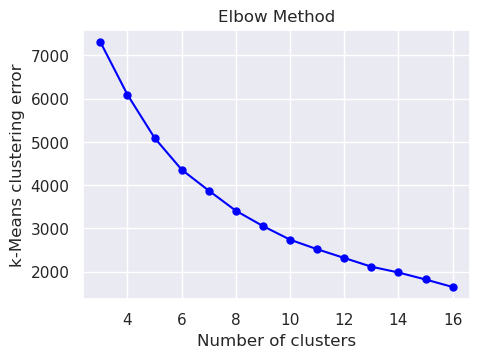
\includegraphics[width=\textwidth]{../figures/plots/section3/k-means_clustering_error.png}
                \caption{K-means Elbow Method}
                \label{fig:kmeans_elbowmethod}
            \end{minipage}
            \hfill
            \begin{minipage}[c]{0.47\textwidth}
                \centering
                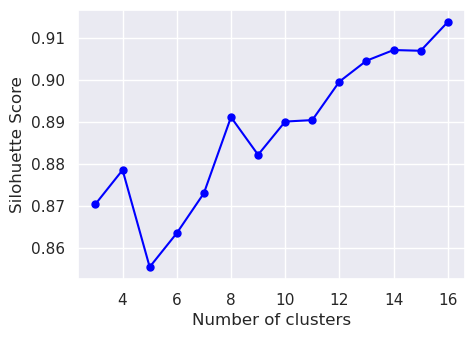
\includegraphics[width=\textwidth]{../figures/plots/section3/k-means_silohuette_score.png}
                \caption{K-means Silhouette Score}
                \label{fig:kmeans_silhouette_score}
            \end{minipage}
        \end{figure}
        
        % \vspace{-0.5cm}
        
        \begin{figure}[h]
            \centering
            \begin{minipage}[c]{0.47\textwidth}
                \centering
                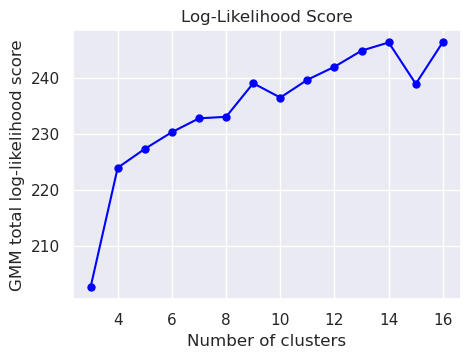
\includegraphics[width=\textwidth]{../figures/plots/section3/gmm_total_log-likelihood_score.png}
                \caption{GMM Log-Likelihood Score}
                \label{fig:gmm_log_likelihood}
            \end{minipage}
            \hfill
            \begin{minipage}[c]{0.47\textwidth}
                \centering
                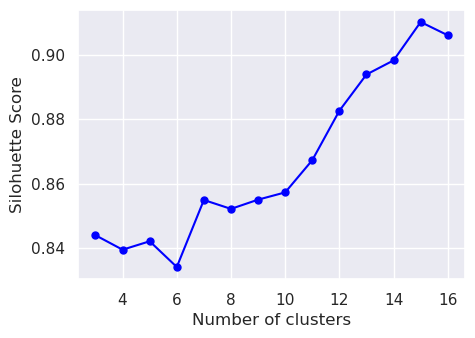
\includegraphics[width=\textwidth]{../figures/plots/section3/gmm_silohuette_score.png}
                \caption{GMM Silhouette Score}
                \label{fig:gmm_silhouette_score}
            \end{minipage}
        \end{figure}

    \subsection{Hyperparameter Tuning}
    
    To optimize both the K-Means and Gaussian Mixture Model (GMM) clustering approaches, hyperparameter tuning was performed using grid search with cross-validation. For K-Means clustering, the optimal parameters identified were:
    \begin{table}[h]
        \centering
        \begin{tabular}{|c|c|c|}
            \hline
            \textbf{Initialization method} & \textbf{Number of initializations (n\_init)} & \textbf{Maximum iterations (max\_iter)} \\
            \hline
            k-means++ & 10 & 50 \\
            \hline
        \end{tabular}
    \end{table}

    The final clustering results achieved a silhouette score of 0.9490 and an inertia value of 1708.96. The high silhouette score indicates well-defined and well-separated clusters, while the minimized inertia suggests an efficient clustering structure. For the Gaussian Mixture Model (GMM), the best hyperparameters found were:
        
        \begin{table}[h]
            \centering
            \begin{tabular}{|c|c|c|c|}
                \hline
                \textbf{Covariance Type} & \textbf{Initialization method} & \textbf{Maximum iterations (max\_iter)} & \textbf{Tolerance (tol)} \\
                \hline
                full & k-means & 50 & 0.001 \\
                \hline
            \end{tabular}
        \end{table}

    The model's performance was evaluated using a silhouette score of 0.9398 and a log-likelihood score of 508.71. Both clustering techniques provided effective segmentation of the dataset. K-Means exhibited a slightly higher silhouette score, suggesting better-defined cluster boundaries, while GMM’s higher log-likelihood highlights its ability to model complex, overlapping clusters.
    \subsection{Clusters Visualization}
    
        To better understand the structure of the clusters, t-SNE dimensionality reduction was applied. While t-SNE is effective for visualizing high-dimensional data, its interpretation must align with clustering validation metrics. 
        
        \begin{figure}[h]
            \centering
            \begin{minipage}[c]{0.47\textwidth}
                \centering
                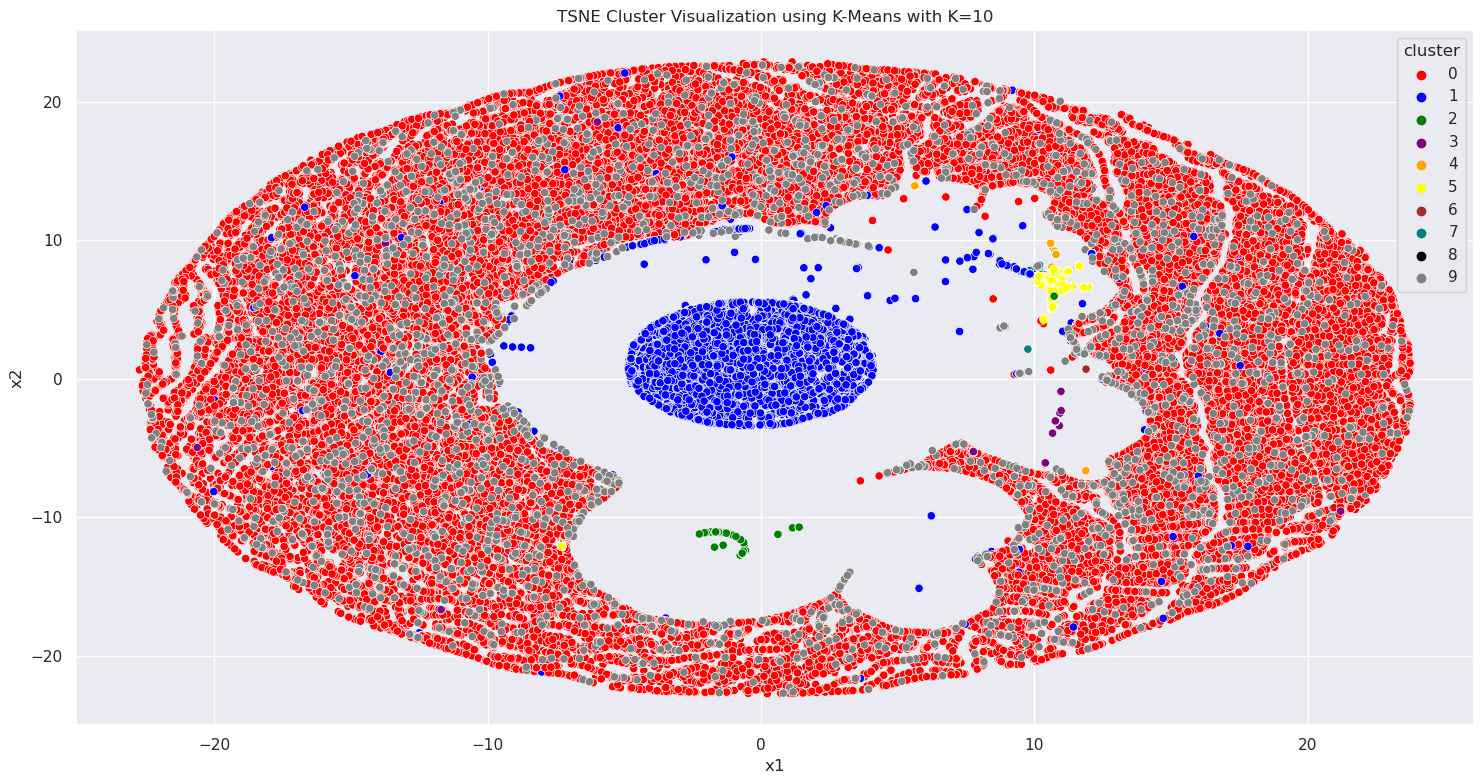
\includegraphics[width=\textwidth]{../figures/plots/section3/tsne_kmeans_clusters.png}
                \caption{t-SNE Visualization of K-Means Clusters}
                \label{fig:tsne_kmeans}
            \end{minipage}
            \hfill
            \begin{minipage}[c]{0.47\textwidth}
                \centering
                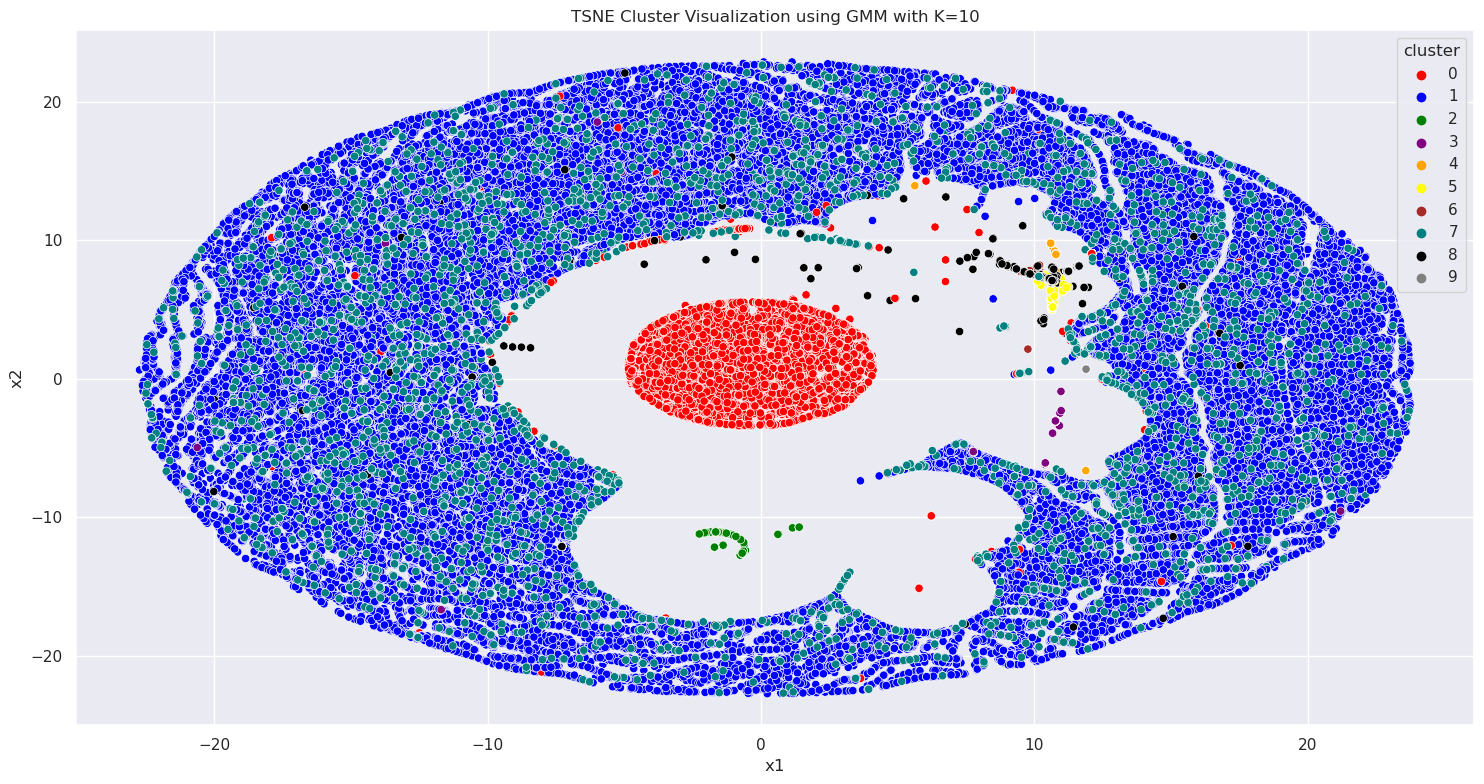
\includegraphics[width=\textwidth]{../figures/plots/section3/tsne_gmm_clusters.png}
                \caption{t-SNE Visualization of GMM Clusters}
                \label{fig:tsne_gmm}
            \end{minipage}
        \end{figure}

        \subsubsection{K-Means Visualization \\}

        The t-SNE visualization of K-Means clustering reveals that a significant portion of the dataset is assigned to a dominant red cluster. While this cluster appears dense, it raises concerns about the method’s ability to differentiate between distinct attack types. The blue and purple clusters are more compact and well-separated, suggesting a few meaningful subgroups. However, several smaller clusters are sparsely distributed, potentially indicating outliers rather than well-formed attack patterns. This visualization suggests that a majority of attacks are grouped together, limiting the effectiveness of this approach.

        \subsubsection{GMM Visualization \\}
        
        The t-SNE visualization of GMM clustering reveals a different structure. Unlike K-Means, which forces strict cluster assignments, GMM probabilistically associates data points with multiple clusters. The resulting visualization displays smoother transitions between clusters, particularly in peripheral areas. However, a large central cluster remains dominant, similar to K-Means. This suggests that while GMM captures more complex attack distributions, it does not necessarily provide significantly better differentiation between attacks. The presence of overlapping points implies that GMM is better suited for identifying gradual variations in attack behaviors rather than strict categorization.

    \subsection{Clusters Analysis}

        \subsubsection{Word Cloud Representation \\}

        Word clouds were generated to highlight the dominant terms in each cluster. However, upon closer inspection, the clusters display a significant degree of overlap in command usage, which raises concerns about the distinctiveness of the attack groupings.
        \begin{itemize}

            \item Many clusters contain commonly used system commands such as \texttt{grep}, \texttt{tmp}, and \texttt{var}, which are present in multiple clusters. This suggests that the clustering process may have grouped sessions based on general command usage rather than clear behavioral differences in attack methodologies. While some clusters, such as Cluster 4 with \texttt{ssh}, \texttt{authorizedkeys}, and \texttt{passwd}, appear indicative of authentication-related activity, most clusters contain highly generic commands that do not necessarily indicate distinct attack types.
            
            \item Clusters 5 and 8, which feature \texttt{chmod}, \texttt{wget}, and \texttt{rm}, could suggest interactions with file systems and downloading behaviors. However, these commands are widely used across many attack types, reducing their effectiveness in defining specific attack categories.
            
            \item Cluster 2, which includes \texttt{busybox} and \texttt{mounts}, is one of the few clusters that might point toward IoT-related attack scenarios, as these commands are frequently used in embedded system environments. However, without additional contextual information, this distinction remains speculative.
            
            \item Cluster 6 contains \texttt{shell}, \texttt{system}, and \texttt{name}, but these terms are too generic to draw meaningful conclusions about a particular type of attack.
            
        \end{itemize}
        Overall, while word clouds provide a useful summary of frequent commands, they do not strongly support the hypothesis that the clusters correspond to clearly defined attack patterns.
            
            \begin{figure}[H]
                \centering
                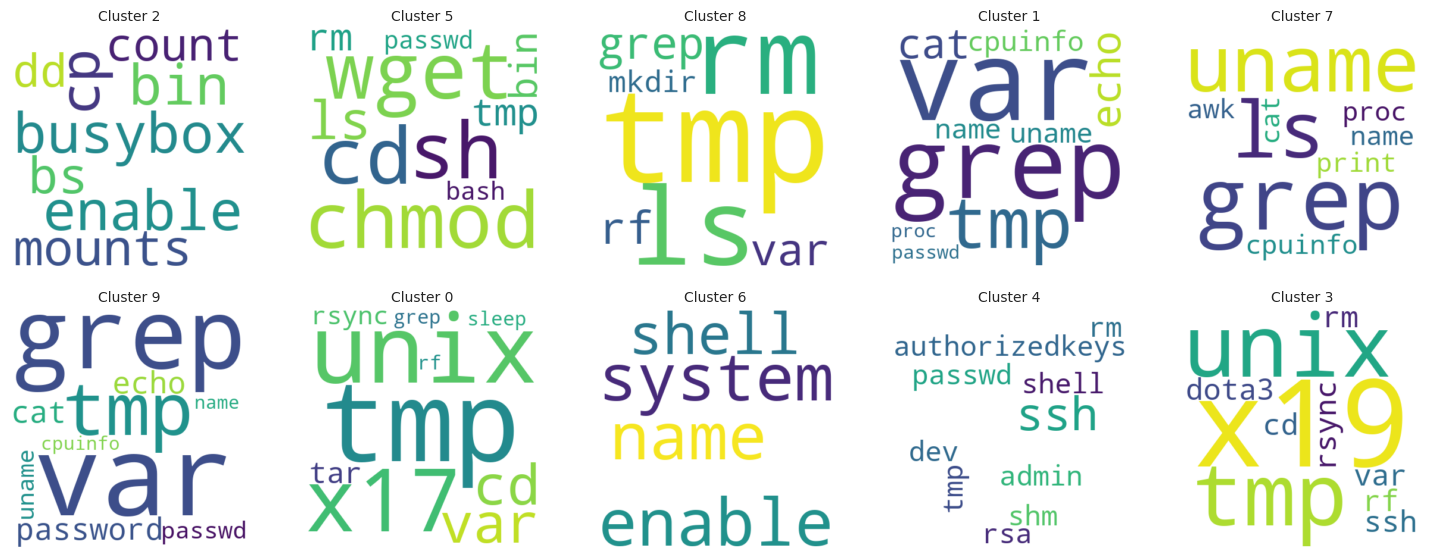
\includegraphics[width=0.9\textwidth]{../figures/plots/section3/circular_wordclouds.png}
                \caption{Word Clouds for Each Cluster}
                \label{fig:word_clouds}
            \end{figure}
            
            \subsubsection{Community Detection \\}
            
                Graph-based community detection was applied to further segment clusters into subgroups. The results indicate that specific communities focus on distinct attack behaviors:

                \begin{itemize}
                    \item The K-Means-based community detection identified well-defined subgroups, but many commands appear across multiple communities, indicating overlapping behaviors.
                    \item The GMM-based community detection aligns with K-Means results, with some additional flexibility in capturing transitional attack patterns. However, the persistence of a dominant cluster in both methods suggests that neither approach fully separates attacks into meaningful, non-overlapping categories.
                \end{itemize}
                
                Overall, while community detection adds another layer of granularity, the results indicate that SSH attack behaviors exhibit significant overlap, making strict segmentation challenging. Additional analysis of the single communities in the appendix. 
                Instead, the overlap in dominant terms suggests that the clustering process may have captured broader system interaction behaviors rather than distinct categories of SSH attack tactics.
                \begin{figure}[h]
                    \centering
                    \begin{minipage}[c]{0.47\textwidth}
                        \centering
                        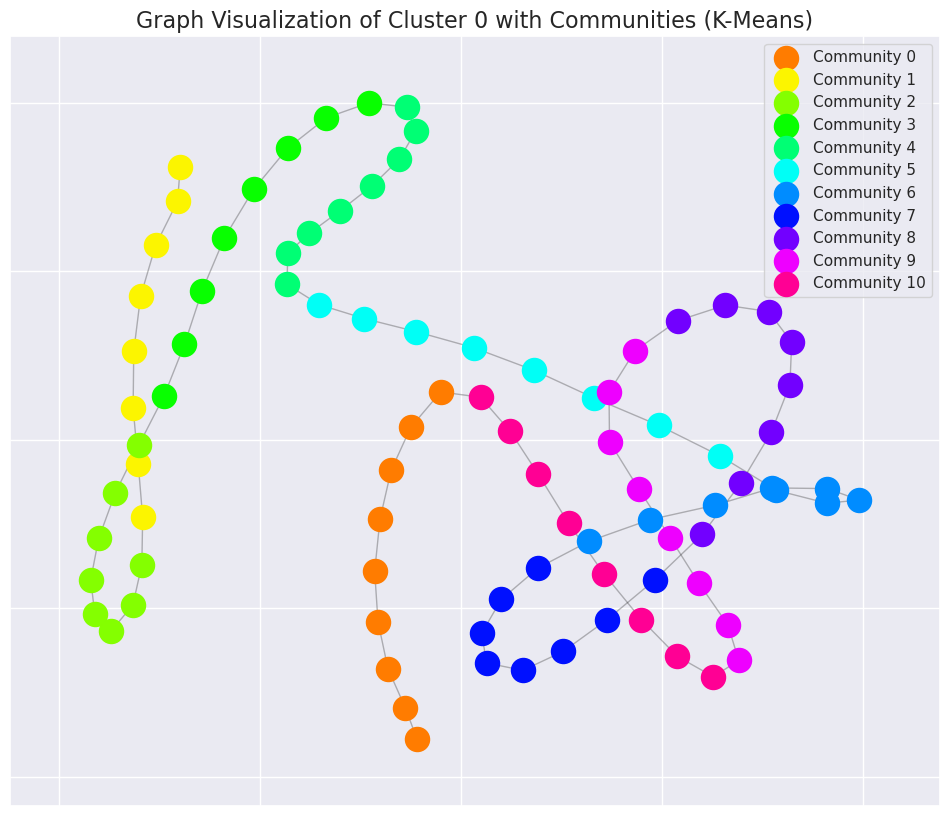
\includegraphics[width=0.8\textwidth]{../figures/plots/section3/k-means_graph_visualization_of_cluster_0_with_communities.png}
                        \caption{Community Detection in Cluster 0 (K-Means).}
                        \label{fig:kmeans_graph}
                    \end{minipage}
                    \hfill
                    \begin{minipage}[c]{0.47\textwidth}
                        \centering
                        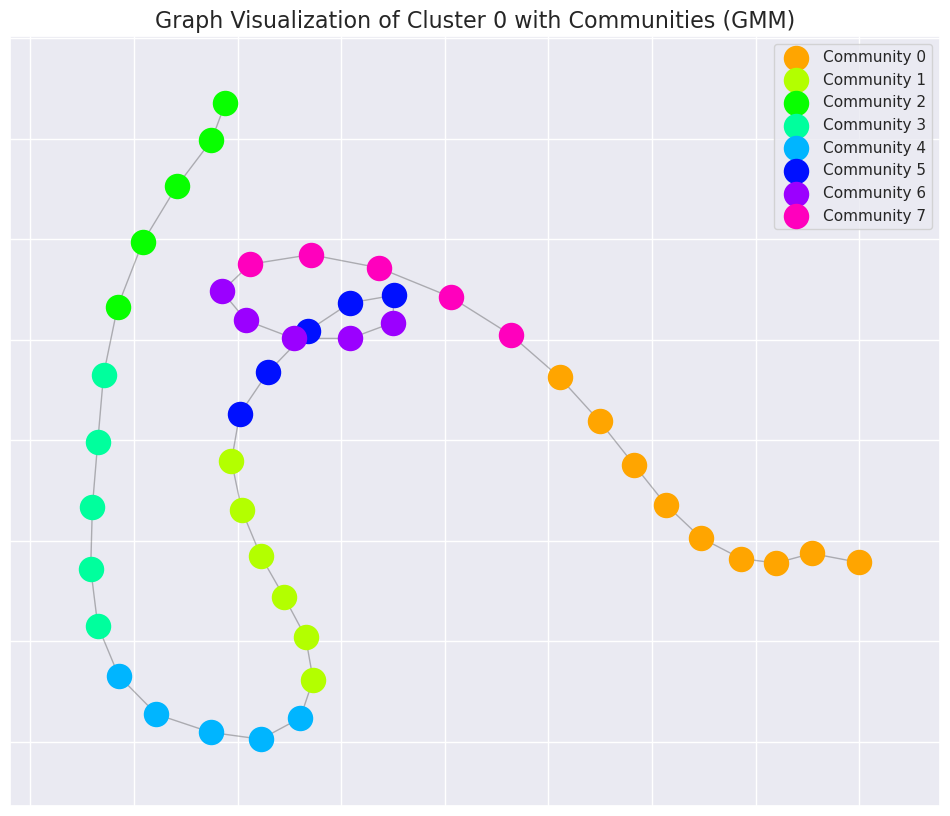
\includegraphics[width=0.8\textwidth]{../figures/plots/section3/gmm_graph_visualization_of_cluster_0_with_communities.png}
                        \caption{Community Detection in Cluster 0 (GMM).}
                        \label{fig:gmm_graph}
                    \end{minipage}
                \end{figure}
            

    \subsection{Conclusion}
        

        This analysis provided insights into SSH attack patterns through clustering, using both K-Means and GMM. While validation metrics and hyperparameter tuning optimized the models, the visualized results indicate significant overlap between clusters, suggesting challenges in achieving well-separated attack groupings. The presence of dominant clusters encompassing much of the dataset hints at either insufficient feature discrimination or limitations in the chosen clustering techniques. Despite these challenges, the study demonstrates the potential of unsupervised learning in revealing underlying structures in SSH attack data, forming a basis for further refinement in cybersecurity threat detection.
        
% 06-language-model-exploration.tex

% Language Models Exploration
% 6.1. Introduction: Provides an overview of the language models task and its objectives.
% 6.2. Pretraining: Describes the process of pretraining Doc2Vec or using a pretrained Bert model.
% 6.3. Model Fine-tuning: Fine-tunes the last layer of the network.
% 6.4. Learning Curves: Plots learning curves and determines the optimal number of epochs.

% Section Title
% \section{Language Model Exploration}
\section{LANGUAGE MODEL EXPLORATION}

    % Main Content
    This section \ldots

    % Subsections
    \subsection{Introduction}
    
        Overview of the language models task and its objectives.

        \ldots

    \subsection{Pretraining}
    
        Pretraining Doc2Vec or using a pretrained Bert model.

        \ldots
        
    \subsection{Model Fine-tuning}
    
        Fine-tuning the last layer of the network.

        \ldots
        
    \subsection{Learning Curves}
    
        Plotting learning curves and determining the optimal number of epochs.

        \ldots

% 07-conclusion.tex

% Conclusion: Summarizing the key findings, challenges, and future work.

% Section Title
\section{CONCLUSION}

    % Main Content

    \subsection{Summary of Key Findings}
    
        In this project, we explored various techniques for analyzing and classifying SSH shell attack logs. The primary objectives were to preprocess the data, perform exploratory data analysis, implement supervised and unsupervised learning models, and leverage advanced language models for classification tasks. Here, we summarize the key findings from each section of the project.

        \textbf{Data Exploration and Pre-processing:} We began by loading and inspecting the dataset, identifying missing values, and handling duplicates. Temporal analysis revealed significant variations in attack frequencies over time, with notable peaks during specific hours and months. Feature extraction and common words analysis provided insights into the most frequent commands and intents used in the attack sessions.

        \textbf{Supervised Learning - Classification:} We implemented and evaluated several machine learning models, including Logistic Regression, Random Forest, and Support Vector Machine (SVM). Hyperparameter tuning improved the performance of these models, and the result analysis highlighted the strengths and weaknesses of each approach.

        \textbf{Unsupervised Learning - Clustering:} Clustering techniques, such as K-Means and Gaussian Mixture Models (GMM), were used to group similar attack sessions. The elbow method and silhouette analysis helped determine the optimal number of clusters. Cluster visualization using t-SNE technique has not provided a clear distincion among the clusters. This could prove that the chosen unsupervised learning models are not suitable for this type of dataset. 

        \textbf{Language Model Exploration:} We explored the use of advanced language models, such as BERT, for classifying attack session tactics. Fine-tuning the pretrained BERT model on our dataset improved classification performance. Learning curves indicated the optimal number of epochs for training, helping to avoid overfitting. 

        \vspace{0.5em} By comparing different types of machine learning techniques and their results, we can understand that, for the applied dataset, a classification methodology based on semantics and LLM can yield more significant results compared to analyzing the same data using basic machine learning technique(unsupervised learning \/ basic classification).

    \subsection{Challenges Faced}
    
        Throughout the project, we encountered several challenges that required careful consideration and problem-solving.

        \textbf{Data Quality and Preprocessing:} Handling missing values, duplicates, and inconsistencies in the dataset was a critical step. Ensuring the data was clean and well-prepared for analysis required significant effort. Additionally, the unstructured nature of the session text posed challenges for text representation and feature extraction.

        \textbf{Model Selection and Tuning:} Selecting appropriate machine learning models and tuning their hyperparameters was a complex task. Balancing model complexity with performance and avoiding overfitting required iterative experimentation and validation.

        \textbf{Computational Resources:} Training advanced language models, such as BERT, required substantial computational resources. Efficiently managing these resources and optimizing the training process was essential to achieve timely results.

        \textbf{Interpretability of Results:} Interpreting the results of clustering and classification models, especially in the context of cybersecurity, was challenging. Ensuring that the findings were meaningful and actionable required careful analysis and domain knowledge.

    \subsection{Future Work}
    
        Based on the findings and challenges encountered in this project, we propose several directions for future work.

        \textbf{Enhanced Feature Engineering:} Further exploration of feature engineering techniques, such as incorporating domain-specific knowledge and using advanced text representation methods, could improve model performance. Experimenting with additional features, such as network metadata and contextual information, may provide deeper insights into attack patterns.

        \textbf{Advanced Model Architectures:} Exploring more advanced model architectures, such as transformer-based models and deep neural networks, could enhance classification accuracy. Transfer learning with other pretrained models and ensemble methods may also yield better results.

        \textbf{Real-time Analysis and Detection:} Implementing real-time analysis and detection systems for SSH shell attacks could provide immediate insights and responses to potential threats. Integrating the models developed in this project into a real-time monitoring framework would be a valuable extension.

        \textbf{Broader Dataset and Generalization:} Expanding the dataset to include a wider range of attack types and sources would improve the generalizability of the models. Collaborating with other organizations to share data and insights could enhance the robustness and applicability of the findings.

    \subsection{Conclusion}
    
        This project demonstrated the potential of machine learning and advanced language models for analyzing and classifying SSH shell attack logs. By leveraging various techniques, we gained valuable insights into attack patterns and behaviors, which can inform cybersecurity strategies and defenses. Despite the challenges faced, the results highlight the importance of data-driven approaches in enhancing cybersecurity threat detection and response capabilities. Future work in this area holds promise for further advancements and practical applications in the field of cybersecurity.


% Include the appendix
% % appendix.tex

\appendix

\section{Appendix}

    \subsection{Code Snippets}

        \subsubsection{Data Exploration and Pre-processing}

            % Load and inspect the dataset
            \begin{lstlisting}[caption={Load and inspect the dataset}, label={lst:load-inspect-dataset}]
                # Load the dataset
                SSH_Attacks = pd.read_parquet("../data/processed/ssh_attacks_decoded.parquet")
        
                # Inspect the dataset structure
                print(SSH_Attacks.info())
        
                # Check for missing values
                print(SSH_Attacks.isnull().sum())
        
                # Check for duplicate rows
                print(SSH_Attacks.duplicated().sum())
            \end{lstlisting}

            % Convert timestamps and analyze frequencies
            \begin{lstlisting}[caption={Convert timestamps and analyze frequencies}, label={lst:convert-analyze-frequencies}]
                # Convert first_timestamp to datetime format
                SSH_Attacks['first_timestamp'] = pd.to_datetime(SSH_Attacks['first_timestamp'])

                # Analyze attack frequencies over time
                temporal_series = (
                    SSH_Attacks.groupby(SSH_Attacks['first_timestamp'].dt.date)
                    .size()
                    .reset_index(name='attack_count')
                )
            \end{lstlisting}

            % Extract and visualize class distribution
            \begin{lstlisting}[caption={Extract and visualize class distribution}, label={lst:extract-visualize-classes}]
                # Extract and count occurrences of each class
                all_classes = SSH_Attacks['Set_Fingerprint'].explode().str.strip()
                class_counts = all_classes.value_counts()

                # Plot the distribution of classes
                sns.barplot(x=class_counts.index, y=class_counts.values, palette='viridis')
            \end{lstlisting}

            % Generate a word cloud from session text
            \begin{lstlisting}[caption={Generate a word cloud from session text}, label={lst:generate-wordcloud}]
                # Generate a word cloud for the session text
                wordcloud = WordCloud(width=800, height=400, background_color='white').generate(' '.join(SSH_Attacks['Full session text']))
                plt.imshow(wordcloud, interpolation='bilinear')
                plt.axis('off')
                plt.show()
            \end{lstlisting}

            % Group attacks by fingerprint and date
            \begin{lstlisting}[caption={Group attacks by fingerprint and date}, label={lst:group-attacks}]
                # Group by Set_Fingerprint and date to count occurrences
                grouped_SSH_Attacks = (
                    SSH_Attacks.explode('Set_Fingerprint')
                    .groupby([SSH_Attacks['first_timestamp'].dt.date, 'Set_Fingerprint'])
                    .size()
                    .reset_index(name='attack_count')
                )
            \end{lstlisting}

            % Convert text into numerical representations
            \begin{lstlisting}[caption={Convert text into numerical representations}, label={lst:convert-text-numerical}]
                # Convert text into numerical representations using Bag of Words (BoW)
                from sklearn.feature_extraction.text import CountVectorizer
                bow_vectorizer = CountVectorizer()
                X_bow = bow_vectorizer.fit_transform(SSH_Attacks['Full session text'])

                # Convert text into numerical representations using TF-IDF
                from sklearn.feature_extraction.text import TfidfVectorizer
                tfidf_vectorizer = TfidfVectorizer()
                X_tfidf = tfidf_vectorizer.fit_transform(SSH_Attacks['Full session text'])
            \end{lstlisting}

        \subsubsection{Supervised Learning - Classification}

            % TODO: add

        \subsubsection{Unsupervised Learning - Clustering}

            % Elbow Method for k-Means Clustering
            \begin{lstlisting}[caption={Elbow Method for k-Means Clustering}, label={lst:elbow_method}]
                # Elbow Method
                n_cluster_list = []
                inertia_list = []
                for n_clusters in range(3, 17):
                    kmeans = KMeans(n_clusters=n_clusters, n_init=10, random_state=42)
                    kmeans.fit(X)
                    inertia_list.append(kmeans.inertia_)
                    n_cluster_list.append(n_clusters)
                
                # Plot Elbow Method
                plt.figure(figsize=(5, 3.5))
                plt.plot(n_cluster_list, inertia_list, marker='o', markersize=5, color='blue')
                plt.xlabel('Number of clusters')
                plt.ylabel('k-Means clustering error')
                plt.title('Elbow Method')
                plt.show()
            \end{lstlisting}

            % Silhouette Analysis for k-Means Clustering
            \begin{lstlisting}[caption={Silhouette Analysis for k-Means Clustering}, label={lst:silhouette_analysis}]
                # Silhouette Analysis
                silhouette_list = []
                for n_clusters in range(3, 17):
                    kmeans = KMeans(n_clusters=n_clusters, n_init=10, random_state=42)
                    labels = kmeans.fit_predict(X)
                    silhouette_score_value = silhouette_score(X, labels)
                    silhouette_list.append(silhouette_score_value)
                
                # Plot Silhouette Analysis
                plt.figure(figsize=(5, 3.5))
                plt.plot(n_cluster_list, silhouette_list, marker='o', markersize=5, color='blue')
                plt.xlabel('Number of clusters')
                plt.ylabel('Silhouette Score')
                plt.title('Silhouette Analysis')
                plt.show()
            \end{lstlisting}

            % Grid Search for k-Means Clustering
            \begin{lstlisting}[caption={Grid Search for k-Means Clustering}, label={lst:grid_search_kmeans}]
                # Define parameter grid for K-Means
                param_grid_kmeans = {
                    'init': ['k-means++', 'random'],
                    'n_init': list(range(10, 21, 2)),
                    'max_iter': list(range(50, 200, 50)),
                }
                
                # Create KMeans object
                kmeans = KMeans(n_clusters=10, random_state=42)
                
                # Create GridSearchCV object
                grid_search_kmeans = GridSearchCV(kmeans, param_grid=param_grid_kmeans, cv=5)
                
                # Fit the grid search to the data
                grid_search_kmeans.fit(X)
                
                # Get the best parameters
                best_params_kmeans = grid_search_kmeans.best_params_
                print("Best parameters:", best_params_kmeans)
            \end{lstlisting}

            % Grid Search for Gaussian Mixture Model (GMM)
            \begin{lstlisting}[caption={Grid Search for Gaussian Mixture Model (GMM)}, label={lst:grid_search_gmm}]
                # Define parameter grid for GMM
                param_grid_gmm = {
                    'init_params': ['kmeans'],
                    'covariance_type': ['full', 'spherical'],
                    'tol': [1e-3, 1e-4, 1e-5],
                    'max_iter': list(range(50, 300, 50)),
                }
                
                # Create GaussianMixture object
                gmm = GaussianMixture(n_components=10, random_state=42)
                
                # Create GridSearchCV object
                grid_search_gmm = GridSearchCV(gmm, param_grid=param_grid_gmm, cv=5, scoring=silhouette_scorer)
                
                # Fit the grid search to the data
                grid_search_gmm.fit(X)
                
                # Get the best parameters
                best_params_gmm = grid_search_gmm.best_params_
                print("Best parameters:", best_params_gmm)
            \end{lstlisting}

            % t-SNE Visualization of Clusters
            \begin{lstlisting}[caption={t-SNE Visualization of Clusters}, label={lst:tsne_visualization}]
                # Apply t-SNE to reduce the number of components
                tsne = TSNE(n_components=2, random_state=42).fit_transform(X)
                df_tsne = pd.DataFrame(tsne, columns=['x1', 'x2'])
                
                # K-Means Clusters
                df_tsne['cluster_kmeans'] = kmeans_tuned.labels_
                sns.scatterplot(data=df_tsne, x='x1', y='x2', hue='cluster_kmeans', palette='viridis')
                plt.title('t-SNE Visualization of K-Means Clusters')
                plt.show()
                
                # GMM Clusters
                df_tsne['cluster_gmm'] = gmm_tuned.predict(X)
                sns.scatterplot(data=df_tsne, x='x1', y='x2', hue='cluster_gmm', palette='viridis')
                plt.title('t-SNE Visualization of GMM Clusters')
                plt.show()
            \end{lstlisting}

            % Feature Distribution Analysis by Cluster
            \begin{lstlisting}[caption={Feature Distribution Analysis by Cluster}, label={lst:feature_distribution}]
                # Analyze the distribution of features within each cluster
                for cluster in range(10):
                    cluster_data = df_tsne[df_tsne['cluster_kmeans'] == cluster]
                    print(f"Cluster {cluster} Feature Distribution:")
                    print(cluster_data.describe())
            \end{lstlisting}

            % Intent Proportions Analysis by Cluster
            \begin{lstlisting}[caption={Intent Proportions Analysis by Cluster}, label={lst:intent_proportions}]
                # Calculate the proportion of each intent within the clusters
                for cluster in range(10):
                    cluster_data = df_tsne[df_tsne['cluster_kmeans'] == cluster]
                    intent_proportions = cluster_data['intent'].value_counts(normalize=True)
                    print(f"Cluster {cluster} Intent Proportions:")
                    print(intent_proportions)
            \end{lstlisting}

            % Attack Categories Analysis by Cluster
            \begin{lstlisting}[caption={Attack Categories Analysis by Cluster}, label={lst:attack_categories}]
                # Analyze the most frequent attack categories within the clusters
                for cluster in range(10):
                    cluster_data = df_tsne[df_tsne['cluster_kmeans'] == cluster]
                    attack_categories = cluster_data['attack_category'].value_counts()
                    print(f"Cluster {cluster} Attack Categories:")
                    print(attack_categories)
            \end{lstlisting}

        \subsubsection{Language Model Exploration}

            % TODO: add


% TODO: check
% Include the bibliography file
\bibliography{../template/column-format-template/sample-base}

% At end of document
% \bibliography{references}           % Single .bib file
% \bibliography{ref1,ref2,ref3}       % Multiple .bib files

\end{document}
